\documentclass[a4paper,11pt]{article}
\usepackage{amsmath,amsthm,amsfonts,amssymb,amscd,amstext,vmargin,graphics,graphicx,tabularx,multicol} \usepackage[french]{babel}
\usepackage[utf8]{inputenc}  
\usepackage[T1]{fontenc} 
\usepackage[T1]{fontenc}
\usepackage{amsmath,amssymb}
\usepackage{pstricks-add,tikz,tkz-tab,variations}
\usepackage[autolanguage,np]{numprint} 
\usepackage{color}
\usepackage{ulem}

\setmarginsrb{1.5cm}{0.5cm}{1cm}{0.5cm}{0cm}{0cm}{0cm}{0cm} %Gauche, haut, droite, haut
\newcounter{numexo}
\newcommand{\exo}[1]{\stepcounter{numexo}\noindent{\bf Exercice~\thenumexo} : \marginpar{\hfill /#1}}
\reversemarginpar


\newcounter{enumtabi}
\newcounter{enumtaba}
\newcommand{\q}{\stepcounter{enumtabi} \theenumtabi.  }
\newcommand{\qa}{\stepcounter{enumtaba} (\alph{enumtaba}) }
\newcommand{\initq}{\setcounter{enumtabi}{0}}
\newcommand{\initqa}{\setcounter{enumtaba}{0}}

\newcommand{\be}{\begin{enumerate}}
\newcommand{\ee}{\end{enumerate}}
\newcommand{\bi}{\begin{itemize}}
\newcommand{\ei}{\end{itemize}}
\newcommand{\bp}{\begin{pspicture*}}
\newcommand{\ep}{\end{pspicture*}}
\newcommand{\bt}{\begin{tabular}}
\newcommand{\et}{\end{tabular}}
\renewcommand{\tabularxcolumn}[1]{>{\centering}m{#1}} %(colonne m{} centrée, au lieu de p par défault) 
\newcommand{\tnl}{\tabularnewline}

\newcommand{\trait}{\noindent \rule{\linewidth}{0.2mm}}
\newcommand{\hs}[1]{\hspace{#1}}
\newcommand{\vs}[1]{\vspace{#1}}

\newcommand{\N}{\mathbb{N}}
\newcommand{\Z}{\mathbb{Z}}
\newcommand{\R}{\mathbb{R}}
\newcommand{\C}{\mathbb{C}}
\newcommand{\Dcal}{\mathcal{D}}
\newcommand{\Ccal}{\mathcal{C}}
\newcommand{\mc}{\mathcal}

\newcommand{\vect}[1]{\overrightarrow{#1}}
\newcommand{\ds}{\displaystyle}
\newcommand{\eq}{\quad \Leftrightarrow \quad}
\newcommand{\vecti}{\vec{\imath}}
\newcommand{\vectj}{\vec{\jmath}}
\newcommand{\Oij}{(O;\vec{\imath}, \vec{\jmath})}
\newcommand{\OIJ}{(O;I,J)}

\newcommand{\bmul}[1]{\begin{multicols}{#1}}
\newcommand{\emul}{\end{multicols}}


\newcommand{\reponse}[1][1]{%
\multido{}{#1}{\makebox[\linewidth]{\rule[0pt]{0pt}{20pt}\dotfill}
}}

\newcommand{\titre}[5] 
% #1: titre #2: haut gauche #3: bas gauche #4: haut droite #5: bas droite
{
\noindent #2 \hfill #4 \\
#3 \hfill #5

\vspace{-1.6cm}

\begin{center}\rule{6cm}{0.5mm}\end{center}
\vspace{0.2cm}
\begin{center}{\large{\textbf{#1}}}\end{center}
\begin{center}\rule{6cm}{0.5mm}\end{center}
}



\begin{document}
\pagestyle{empty}
\titre{Contrôle : Calcul littéral, aire et volume}{Nom}{Prénom}{Date}{Classe}
\vspace*{0.5cm}


\begin{flushleft}
\begin{tabular}{|m{6cm}|m{2.5cm}|m{2.5cm}|m{2.5cm}|m{2.5cm}|}
\hline 
\textbf{Compétences} & \begin{center}
\textbf{Très bonne maîtrise}
\end{center} & \begin{center}
\textbf{Maîtrise satisfaisante}
\end{center}  & \begin{center}
\textbf{Maîtrise faible}
\end{center} & \begin{center}
\textbf{Maîtrise insuffisante}
\end{center} \\ 
\hline 
Savoir développer une expression littérale &  &  & &\\
\hline
Savoir factoriser une expression littérale &  &  & & \\ 
\hline
Connaître les formules permettant de calculer les aires et les volumes des figures usuelles &  &  &  &\\ 
\hline 
Savoir calculer le volume de figures composées  &  &  &  &\\ 
\hline 


\end{tabular} 
\end{flushleft}

\vspace*{0.5cm}

\exo{3} Factoriser les expressions suivantes :\\

$A = (x + 5) (4x - 2) - (x + 5) (9x - 1)$	\hspace*{1cm}	$B = 100x^{2} - 60x + 9$ \hspace*{1cm} $C = 81 - 36x^{2}$\\

\vspace*{0.5cm}


\exo{3,5}\\

Dans cet exercice, on utilise le programme de calcul ci-dessous :\\

\bi
\item	choisir un nombre x ,\\
\item	retrancher 3 au double de x ,\\
\item	élever le résultat au carré ,\\
\item	retrancher 16 au résultat obtenu.\\
\ei


\q Si on choisit 5, quel résultat final obtient-on ? Détailler les calculs.\\

\q 	Indiquer, parmi les expressions suivantes, celle qui décrit le programme de calcul donné :

	\begin{center}
	$ A = 2x - 3^{2} -16$ \hspace*{2cm} $C= (2x-3) \times 2 -16$ \hspace*{2cm} $ E= (2x-3)^{2} - 16$\\
	
$B= [(x-3) \times 2]^{2} - 16$	\hspace*{1.75cm} $D =16 - [2 \times (x-3)]$ \hspace*{1.75cm} $F=(3x-16)^{2}$ - 2\\
	\end{center}

\q	Développer et réduire F.\\

\q	Factoriser E.\\



\exo{4} L'unité de longueur est le centimètre. Donner le nom des solides ci-dessous et déterminer leur volume au centième près.\\

\qa \includegraphics[scale=0.8]{vol4.eps} \hspace*{0.7cm} \qa 
\includegraphics[scale=0.8]{vol1.eps} \hspace*{0.7cm} \qa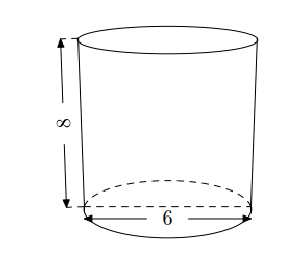
\includegraphics[scale=0.8]{vol2.eps} \hspace*{0.7cm} \qa 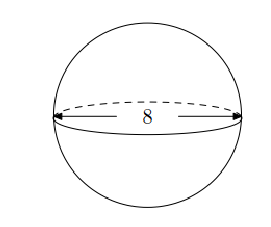
\includegraphics[scale=0.8]{vol3.eps} \\

\newpage

\vspace*{0.5cm}

\exo{3.5}

\bmul{2}

On considère la pyramide ABCD de hauteur [AD] telle que AD = 5 cm et de base ABC telle que AB = 4,8 cm ; BC = 3,6 cm ; CA = 6 cm. \\
(La figure n'est pas aux dimensions.)

\columnbreak

\begin{center}
\includegraphics[scale=1]{volpyramide.eps} 
\end{center}

\emul

\noindent \initq \q Démontrer que le triangle ABC est rectangle en B.\\
\q Calculer le volume de cette pyramide au centième près.\\
\q On désire fabriquer de telles pyramides en plâtre. Combien peut-on en obtenir avec 1 $dm^{3}$ de plâtre ?\\
\vspace*{0.5cm}

\exo{4}

\bmul{2}

Le culbuto ci-contre est un jouet pour enfant qui oscille sur une base sphérique.\\

\initq \q Calculer son volume et donner l'arrondi au $cm^{3}$.\\

\columnbreak

\begin{center}
\includegraphics[scale=1]{culbuto.eps} 
\end{center}

\emul

\q On souhaite peindre en rouge la base sphérique. Calculer l'aire de la surface à peindre. 
En donner la valeur exacte, puis l'arrondi au $cm^{2}$.\\
(\textbf{\underline{Rappel} :} Aire d'une sphère = $4  \pi r^{2}$ )\\

\q Sachant que 1 L de peinture peut couvrir 5,5 $m^{2}$, combien de culbutos pourra-t-on peindre avec un pot de 2,5 L ?\\


\vspace*{0.5cm}



\exo{4}

\bmul{2}

Une boîte de forme parallélépipédique contient trois balles de tennis comme indiqué dans la figure ci contre. Les balles sont en contact avec les côtés de la boîte.\\

\initq \q	Calculer le diamètre d'une balle.\\

\q	Calculer le volume $V_{1}$ de la boîte.\\


\columnbreak

\begin{center}
\includegraphics[scale=1]{exovol.eps} 
\end{center}

\emul


\q Calculer le volume $V_{2}$ des 3 balles, donner l'arrondi au $mm^{3}$.\\

\q	Calculer le pourcentage, arrondi à l'unité, du volume de la boîte occupé par les balles.\\




\end{document}
